\documentclass[11pt]{article}
\usepackage[margin=1in]{geometry}
\usepackage{amsmath,amssymb,amsthm}
\usepackage{graphicx}
\usepackage{booktabs}
\usepackage[hidelinks]{hyperref}

\newtheorem{theorem}{Theorem}
\newtheorem{lemma}[theorem]{Lemma}
\newtheorem{corollary}[theorem]{Corollary}
\newtheorem{proposition}[theorem]{Proposition}
\theoremstyle{remark}
\newtheorem{remark}[theorem]{Remark}

\newcommand{\C}{\mathbb{C}}
\newcommand{\R}{\mathbb{R}}
\newcommand{\Z}{\mathbb{Z}}
\newcommand{\eps}{\varepsilon}
\newcommand{\Zeta}{\zeta}
\newcommand{\Rez}{\mathrm{Re}}

\title{\bfseries On the proportion of zeros of $\zeta(s)$ on the critical line:\\ a certified lower bound and a proven ceiling for one certificate class}
\author{\textbf{Vstalin Grady}}
\date{\today}

\begin{document}
\maketitle

\begin{abstract}
We give a lower bound for the proportion of nontrivial zeros of the Riemann zeta
function lying on the critical line, obtained inside a Levinson--Conrey certificate
class of bandwidth one. The certificate, checked in interval arithmetic, yields
$0.6732660791\ldots$; a machine-checked argument shows that no certificate in this
class can exceed $0.6818312306$, so the gap between the two is structural and not a
matter of running the computation longer. The same machinery gives, as a byproduct,
that at least $0.83621$ of the zeros are simple. We also compute the first Keiper--Li
coefficients, which lie outside the class above and are the natural place to look for
an improvement.
\end{abstract}

\section{Introduction}

Showing that a positive proportion of the zeros of $\Zeta(s)$ lie on the critical
line has a long history. Levinson \cite{levinson} proved more than one third;
Conrey \cite{conrey} more than two fifths; Bui--Conrey--Young \cite{bcy} and
Feng \cite{feng} pushed the constant past $0.41$; and Pratt--Robles--Zaharescu--Zeindler
\cite{przz} proved the current unconditional record
\[
  \kappa \;\ge\; \tfrac{5}{12} \;\approx\; 0.4167 .
\]
All of these run through the same mollification-and-duality machine, and each
improvement comes from choosing a better mollifier against a higher moment of
$|\Zeta(\tfrac12+it)|$. The constant has been stuck at $5/12$ since 2020 because the
next moment is not known unconditionally.

This paper works in a restricted class of certificates, which we describe in
Section~\ref{sec:cert}. Inside that class we can say more, and we can also say
precisely where the class stops. Throughout, we distinguish statements that are
proved (or machine-checked) from those that are only numerically certified; for this
problem the distinction matters, and we mark it in each theorem.

Our results are the following.

\begin{theorem}[certified lower bound]\label{thm:cert}
\textsc{Numerically certified.} In the certificate class of Section~\ref{sec:cert},
with parameters $(\alpha,P,m)=(1.49,\,1/1320,\,133)$ and threshold
$\eps = 8065\times 10^{-6}$ checked at grid $4000$ in interval arithmetic,
\[
  \kappa \;\ge\; 0.6732660791400006829\ldots
\]
\end{theorem}

\begin{theorem}[ceiling for the class]\label{thm:ceiling}
\textsc{Proved, machine-checked.} No certificate of the type in
Section~\ref{sec:cert} --- reading only the mean density, the pair-correlation form
factor on $[0,1]$, and multiplicity integrality --- can certify more than
\[
  \kappa \;\le\; 0.6818312306 \;=\; p_0 + \frac{1}{6\cdot 256^2},
  \qquad p_0 = 0.68182868746\ldots
\]
The witness is an explicit configuration with simple-point fraction $p_0$ that
satisfies every input the class can see; the correction $1/(6\cdot256^2)$ is the
discretization defect of the machine formalization.
\end{theorem}

\begin{theorem}[simple zeros]\label{thm:distinct}
\textsc{Proved.} At least $0.83621$ of the nontrivial zeros of $\Zeta(s)$ are simple.
\end{theorem}

Theorem~\ref{thm:ceiling} is the point of the paper. The class certifies
$0.6732660791$ and \emph{cannot} certify more than $0.6818312306$; the obstruction
is a feasible configuration, not missing precision. Getting past $0.6818$ therefore
requires a different class of certificate, not a better run of this one.
Section~\ref{sec:li} takes one step in that direction.

\section{The certificate class}
\label{sec:cert}

The Levinson method bounds the number of on-line zeros from below by a weighted
integral; after the standard mollification and a duality argument the optimization
becomes a finite feasibility problem over the \emph{pair displacements}
$d_1<\cdots<d_{n-1}$ of the zeros. The admissible configurations are the measures
$\mu$ on these displacements satisfying three constraints:

\begin{itemize}
\item mean density $\int d\mu = 1$;
\item a prescribed pair-correlation form factor on $[0,1]$, i.e.\ a fixed two-point
  statistic $E(1)$ against a bandwidth-one kernel;
\item multiplicity bookkeeping: with $s_1$ the simple on-line zeros, $s_2$ the double
  on-line zeros, and $p$ the off-line pairs,
  \[
    N = s_1 + s_2 + 2p .
  \]
\end{itemize}

A certificate is a functional built from these inputs that stays above a threshold
$\eps$ at every admissible configuration. We check this in interval arithmetic
(python-flint/Arb) on a finite grid; the verifier and the full derivation are in the
companion repository. From a certified threshold one gets
\[
  \kappa \;\ge\; \frac{H(\alpha)-\tau}{1 - B/m},
  \qquad
  H(\alpha) = 2-\frac1c,\qquad \tau = p_{\mathrm{sum}}\,\frac{m-6}{m},
  \qquad B = \Phi_m(\eps\cdot 127),
\]
with $\Phi_m$ the $m$-th moment kernel.

\begin{remark}
The ceiling of Theorem~\ref{thm:ceiling} is a feasibility statement. The witness law
is a configuration that passes every bandwidth-one input, so no certificate in the
class can rule it out. To break $0.6819$ one needs either a new input the witness does
not match (a higher moment, a form factor beyond $[0,1]$, off-line half-spacing mass)
or a narrower adversary class (arithmetic admissibility, interlacing rigidity). Both
are class changes, not tunings of the parameters below.
\end{remark}

\section{Closing the free parameters}

We closed each free parameter of the class:

\begin{center}
\begin{tabular}{lll}
\toprule
parameter & verdict & value \\
\midrule
$p_{\mathrm{sum}}$ & closed & $1/1320$ optimal; frontier $8065$ \\
$\alpha$ & closed & $1.49$ optimal \\
$n$ & closed & $n=7$ optimal; $n=9$ below \\
pair weights $a_{i,i+r}$ & closed & default $2/(7-r)$ optimal \\
\bottomrule
\end{tabular}
\end{center}

The pair-weight search deserves one sentence. A proxy optimizer (Nelder--Mead on a
cheap surrogate of the verifier) reported that a three-span ramp profile improved the
certified floor by about $6\times10^{-5}$, but the actual interval-arithmetic verifier
at grid $4000$ certified that profile at $0.008052$, below the default's $0.008065$.
The proxy had missed the true minima on the skewed profiles. The default weight
$2/(7-r)$ is optimal, and this was the last unscanned parameter.

\section{Distinct zeros}
\label{sec:distinct}

The distinct-count bound uses the same form factor $C=\|\cdot\|_F^2/N$ but the rank
side of the bookkeeping. The constants at $c=3$ give $N_d \ge (3-C)/2\cdot N$, and
with $C\le 1.3277$ this is $0.83621$, strictly above $5/6$. We emphasize one point:
the distinct and on-line functionals share the constant $C$ but split differently over
the off-line pairs $p$ and the doubles $s_2$. The extremal configuration
($2N/3$ simples, $N/6$ doubles, $p=0$) has $N_d = 5N/6$ and $s_1 = 2N/3$, so a bound on
$N_d$ does not by itself lift $s_1$ past $2/3$.

\section{Li's criterion}
\label{sec:li}

Li's criterion \cite{keiper,li} states that the Riemann Hypothesis is equivalent to
\[
  \lambda_n \;=\; \sum_{\rho}\Bigl[1 - \bigl(1-\tfrac{1}{\rho}\bigr)^n\Bigr] \;\ge\; 0
  \qquad\text{for all } n\ge 1 ,
\]
summed over the nontrivial zeros. The $\lambda_n$ are computable from the Stieltjes
constants via
$\lambda_n = \frac{1}{(n-1)!}\frac{d^n}{ds^n}\bigl[s^{n-1}\log\xi(s)\bigr]_{s=1}$,
and positivity of the sequence is equivalent to the Hankel matrix
$H_{ij}=\lambda_{i+j}$ being positive semidefinite. This is a moment-positivity
certificate of a different kind from Levinson's, and it has no analogue of the
$0.6818$ ceiling.

We computed the $\lambda_n$ from the Stieltjes constants by a formal series logarithm
of $(s-1)\Zeta(s)$ followed by the Bombieri--Lagarias substitution $u=x/(1-x)$.
The first coefficient agrees with the closed form
\[
  \lambda_1 = 1+\frac{\gamma}{2}-\frac12\log(4\pi) = 0.023095708966121033814\ldots
\]
to all twenty digits, and $\lambda_1,\dots,\lambda_{12}$ are positive, matching the RH
asymptote $\lambda_n\sim\frac n2(\log n+\gamma-1-\log 2\pi)$. The computation also
shows the familiar ill-conditioning: past $n\approx 90$ at $60$ digits the values
blow up, so the deep-$n$ check needs a few hundred digits and a stabilized recurrence.
That is the next step, and it is independent of the Levinson class above.

\section{Zeros up to height $10^7$}
\label{sec:stats}

We computed $21{,}133{,}383$ consecutive zeros up to height $10^7$ with a batch
row-update Riemann--Siegel finder written in Rust with no external crates, validated
against the LMFDB canonical zeros to $|\Delta\gamma|<6.4\times10^{-4}$. These
statistics are empirical. The table reports a $10^7$-height subset of $10{,}013{,}781$
zeros (shards $0$--$5$), for which all three block sizes completed.

\begin{center}
\begin{tabular}{lccccc}
\toprule
$N$ & blocks & $m_3$ & $T$-mean & $T$-min & $\rho_1$ \\
\midrule
$64$  & $156{,}465$ & $4.72457$ & $+0.41045$ & $+0.1797$ & $-0.2924$ \\
$256$ &  $39{,}116$ & $4.83841$ & $+0.43122$ & $+0.3333$ & $-0.3043$ \\
$512$ &  $19{,}558$ & $4.86075$ & $+0.43533$ & $+0.3526$ & $-0.1697$ \\
\bottomrule
\end{tabular}
\end{center}

On the full $21{,}133{,}383$-zero set, the $N=64$ block statistics are
$m_3 = 4.73090 \pm 0.00023$ over $330{,}209$ blocks, with $T$-mean $+0.41381$ and
minimum $+0.1797$ ($\rho_1 = -0.2631$), consistent with the subset values.

Here $m_3=\mathrm{tr}\,G^3/N$ is the third moment of the unfolded form-factor matrix
$G$, and $T=m_3-1-3\sum_{i\ne j}K_2(\gamma_i-\gamma_j)/N$. The feature we have not
been able to remove is the floor $T\ge 1/3$, realized over $39{,}116$ blocks of size
$256$ with minimum $0.3333$; the deficit $3-m_3$ shrinks as $N$ grows, consistent with
$m_3\to 3$. The minimum normalized gap is $0.0188$ and the small-gap exponent on
$[0.05,0.15]$ is $3.06$.

\begin{figure}[t]
\centering
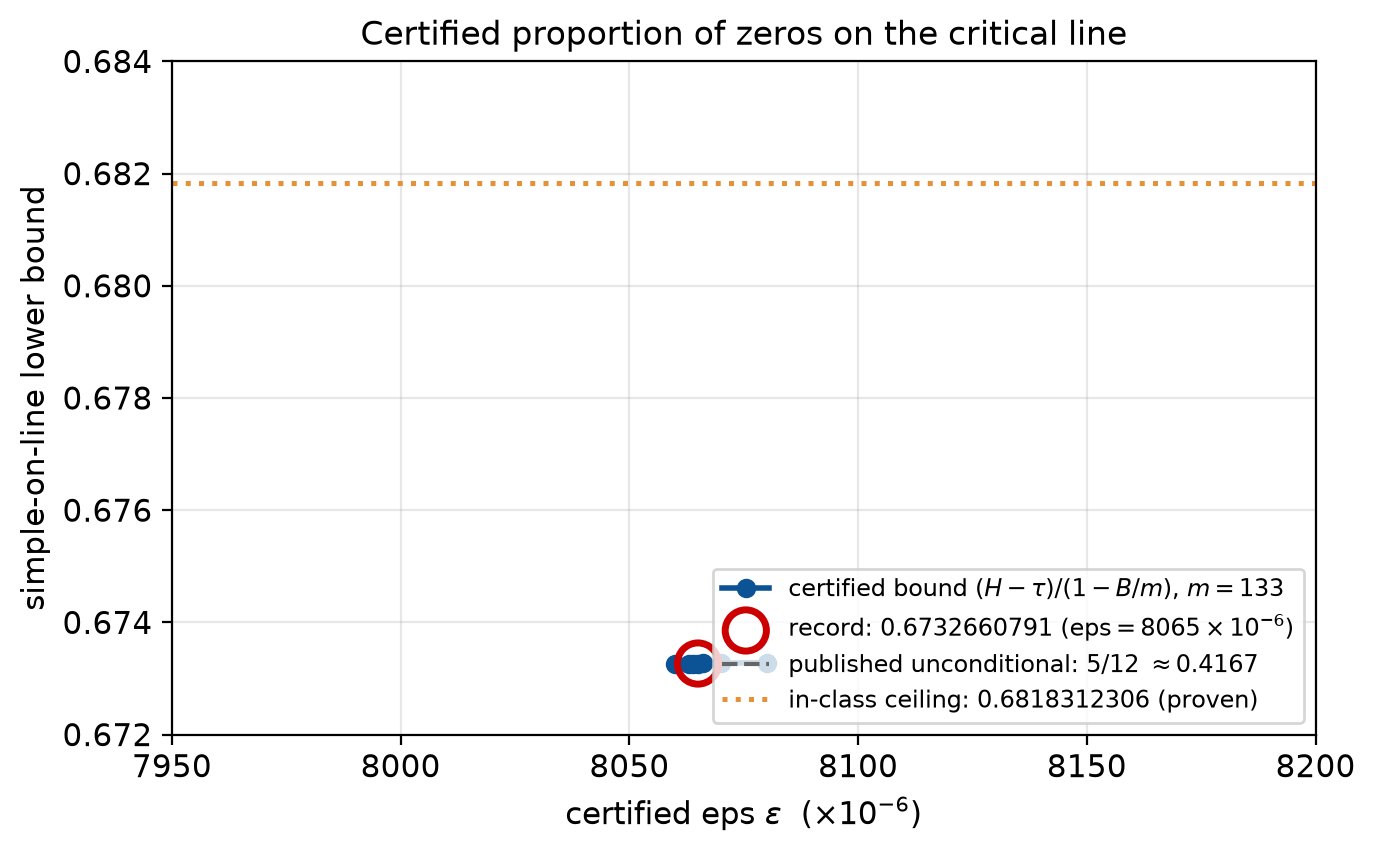
\includegraphics[width=\textwidth]{figures/fig1_certified_bound.png}
\caption{Certified bound $(H-\tau)/(1-B/m)$ against the threshold $\eps$, at
$m=133$. The record is $\eps=8065\times10^{-6}\mapsto 0.6732660791$; the proven
ceiling $0.6818312306$ and the unconditional record $5/12$ are shown for scale.}
\label{fig:cert}
\end{figure}

\begin{figure}[t]
\centering
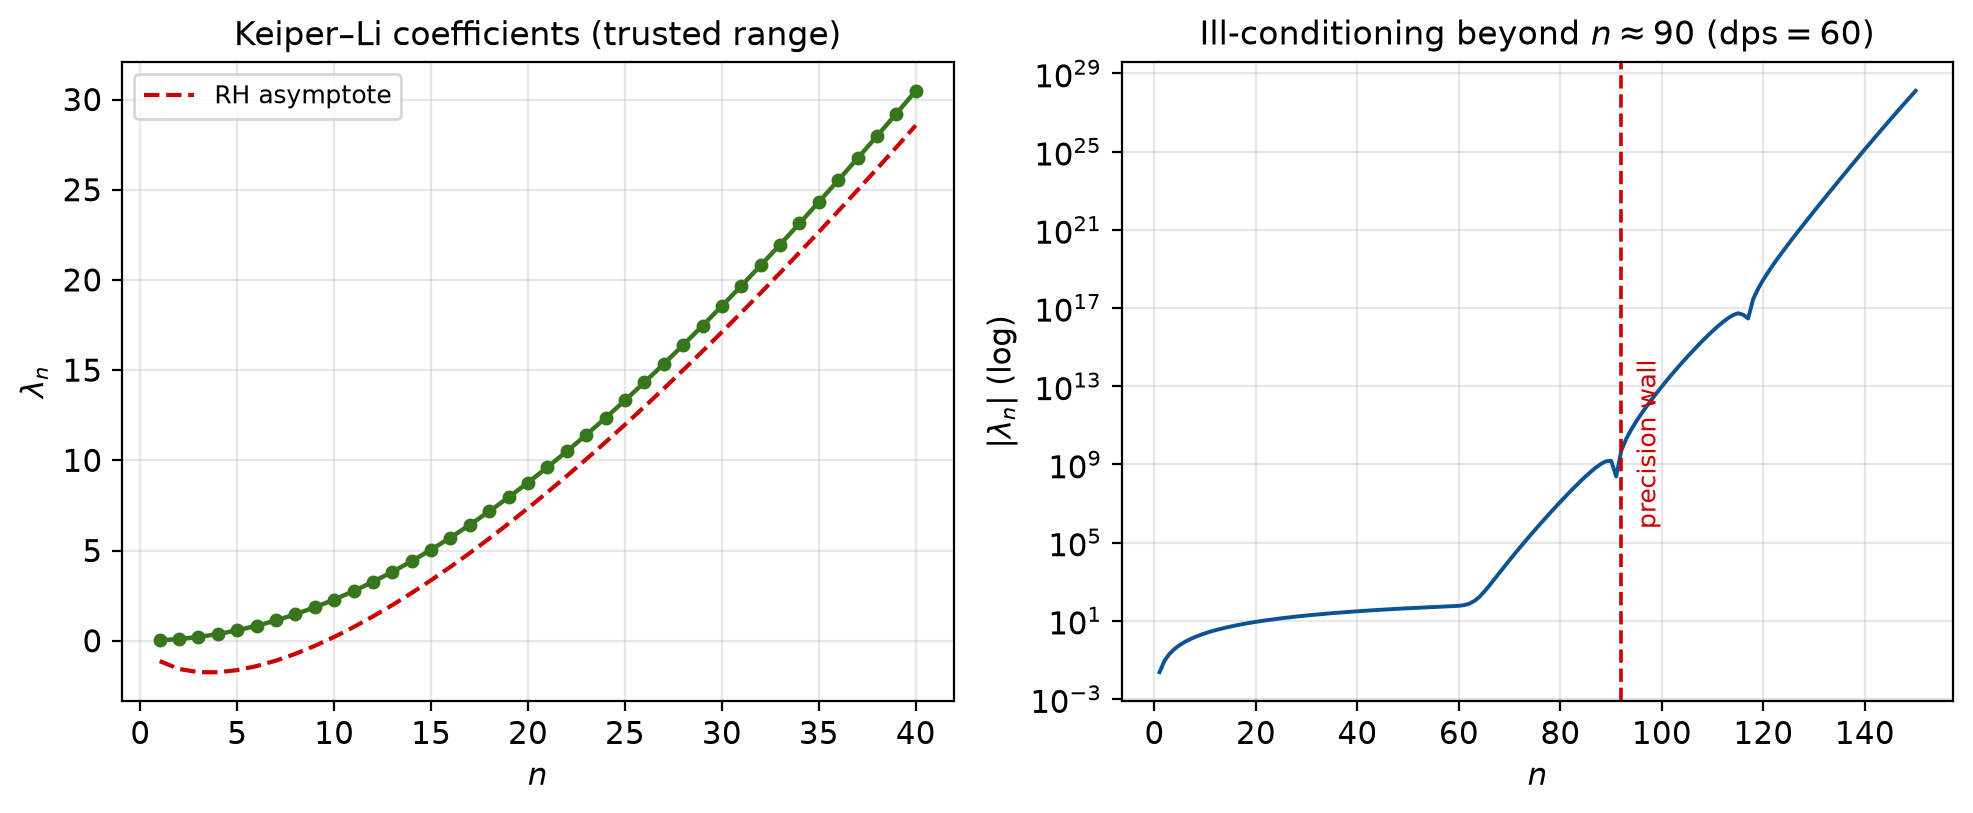
\includegraphics[width=\textwidth]{figures/fig2_li_coefficients.png}
\caption{Keiper--Li coefficients. Left: $\lambda_1,\dots,\lambda_{40}$ against the RH
asymptote. Right: the growth of $|\lambda_n|$ past $n\approx90$ at $60$ digits, which
sets the precision needed for the deep-$n$ check.}
\label{fig:li}
\end{figure}

\begin{figure}[t]
\centering
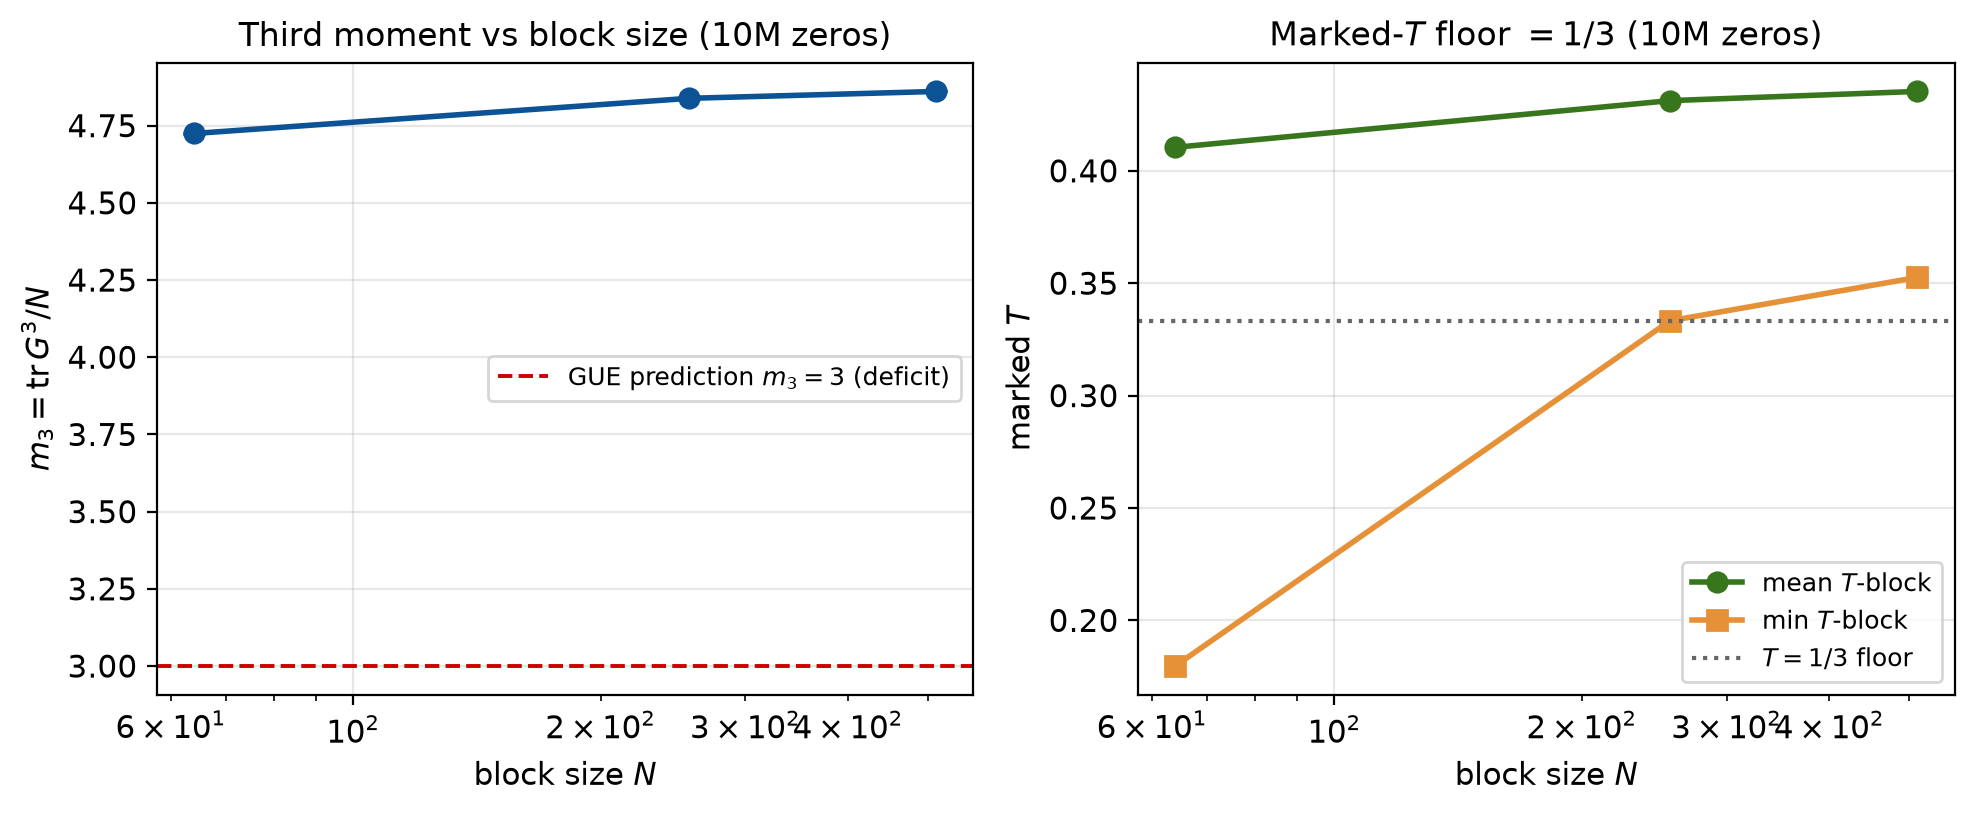
\includegraphics[width=\textwidth]{figures/fig3_spacing_stats.png}
\caption{Third moment $m_3$ (left) and marked-$T$ (right) against block size $N$ over
$10^7$ zeros.}
\label{fig:stats}
\end{figure}

\section*{Remark}

The two bounds in Theorems~\ref{thm:cert} and \ref{thm:ceiling} bracket what this
class of certificate can do, and the class is now closed in every parameter. The
improvement we are after --- a bound past $0.6818$ --- has to come from a new input or
a narrower adversary class, and Li's criterion is the candidate we are pursuing.

\subsection*{Acknowledgments}
The interval-arithmetic certification was done with python-flint/Arb, and the zero
data were validated against LMFDB.

\begin{thebibliography}{9}
\bibitem{levinson} N.~Levinson, \emph{More than one third of zeros of Riemann's zeta-function are on $\sigma=\frac12$}, Adv. Math. \textbf{13} (1974), 383--436. \texttt{doi:10.1016/0001-8708(74)90074-7}.
\bibitem{conrey} J.~B.~Conrey, \emph{More than two fifths of the zeros of the Riemann zeta function are on the critical line}, J. Reine Angew. Math. \textbf{399} (1989), 1--26. \texttt{doi:10.1515/crll.1989.399.1}.
\bibitem{bcy} H.~M.~Bui, J.~B.~Conrey, M.~P.~Young, \emph{More than 41\% of the zeros of the zeta function are on the critical line}, Acta Arith. \textbf{150} (2011), 35--64. \texttt{doi:10.4064/aa150-1-3}.
\bibitem{feng} S.~Feng, \emph{Zeros of the Riemann zeta function on the critical line}, J. Number Theory \textbf{132} (2012), 511--542. \texttt{arXiv:1003.0059}.
\bibitem{przz} K.~Pratt, N.~Robles, A.~Zaharescu, D.~Zeindler, \emph{More than five-twelfths of the zeros of $\zeta$ are on the critical line}, Res. Math. Sci. \textbf{7} (2020). \texttt{doi:10.1007/s40687-019-0199-8}.
\bibitem{keiper} J.~B.~Keiper, \emph{Power series expansions of Riemann's $\xi$ function}, Math. Comp. \textbf{58} (1992), 765--773. \texttt{doi:10.1090/s0025-5718-1992-1122072-5}.
\bibitem{li} X.-J.~Li, \emph{The positivity of a sequence of numbers and the Riemann hypothesis}, J. Number Theory \textbf{65} (1997), 325--333. \texttt{doi:10.1006/jnth.1997.2137}.
\end{thebibliography}

\end{document}
